% answers.tex —— 2004 年·全国卷Ⅰ·文科 · 参考答案与详细解析片段
% 由 tools/generate_projects.py 依来源总账自 2004/2004_数学真题_全国1文_试题.md + 2004/2004_数学真题_全国1文_解析正文.md + 2004/2004_数学真题_全国1文_答案要点.md 生成，勿手改（改源 MD 后重跑）


\begin{gktip}
固定源 PDF 为印刷页码 184–185 的两页题面，不附答案。以下解析均依据固定源独立复算；第 21 题图形在 LaTeX 工程中以 TikZ/PGFPlots 矢量源重绘。
\end{gktip}

\begin{answer}
\gksolhead{1}{}

\textbf{题目}：

设集合 $U=\{1,2,3,4,5\}$，$A=\{1,2,3\}$，$B=\{2,5\}$，则 $A\cap(\complement_U B)=$\mbox{（　　）}

（A）$\{2\}$　　（B）$\{2,3\}$　　（C）$\{3\}$　　（D）$\{1,3\}$

\Needspace{4\baselineskip}
\textbf{解析}

\Needspace{5\baselineskip}
$\complement_U B=\{1,3,4\}$，所以

\nopagebreak[4]
\[
A\cap(\complement_U B)=\{1,3\}.
\]

\gkanswer{答案：D}

\end{answer}
\begin{answer}
\gksolhead{2}{}

\textbf{题目}：

已知函数 $f(x)=\lg\dfrac{1-x}{1+x}$，若 $f(a)=\dfrac12$，则 $f(-a)=$\mbox{（　　）}

（A）$\dfrac12$　　（B）$-\dfrac12$　　（C）$2$　　（D）$-2$

\Needspace{4\baselineskip}
\textbf{解析}

\Needspace{5\baselineskip}
在定义域内有

\nopagebreak[4]
\[
f(-x)=\lg\frac{1+x}{1-x}=-\lg\frac{1-x}{1+x}=-f(x).
\]

故 $f(-a)=-\dfrac12$。

\gkanswer{答案：B}

\end{answer}
\begin{answer}
\gksolhead{3}{}

\textbf{题目}：

已知 $\boldsymbol a\text{、}\boldsymbol b$ 均为单位向量，它们的夹角为 $60^\circ$，那么 $|\boldsymbol a+3\boldsymbol b|=$\mbox{（　　）}

（A）$\sqrt7$　　（B）$\sqrt{10}$　　（C）$\sqrt{13}$　　（D）$4$

\Needspace{4\baselineskip}
\textbf{解析}

\Needspace{5\baselineskip}
由向量夹角公式，

\nopagebreak[4]
\[
|\boldsymbol a+3\boldsymbol b|^2
=|\boldsymbol a|^2+9|\boldsymbol b|^2+6\boldsymbol a\cdot\boldsymbol b
=1+9+6\cos60^\circ=13.
\]

因此 $|\boldsymbol a+3\boldsymbol b|=\sqrt{13}$。

\gkanswer{答案：C}

\end{answer}
\begin{answer}
\gksolhead{4}{}

\textbf{题目}：

函数 $y=\sqrt{x-1}+1$（$x\geqslant1$）的反函数是\mbox{（　　）}

（A）$y=x^2-2x+2$（$x<1$）　　（B）$y=x^2-2x+2$（$x\geqslant1$）

（C）$y=x^2-2x$（$x<1$）　　（D）$y=x^2-2x$（$x\geqslant1$）

\Needspace{4\baselineskip}
\textbf{解析}

\Needspace{5\baselineskip}
令原函数中的自变量为 $u$、函数值为 $v$，则

\nopagebreak[4]
\[
v=\sqrt{u-1}+1
\Longrightarrow
u=(v-1)^2+1=v^2-2v+2.
\]

\Needspace{5\baselineskip}
原函数值域为 $v\geqslant1$，交换字母后反函数为

\nopagebreak[4]
\[
y=x^2-2x+2,\qquad x\geqslant1.
\]

\gkanswer{答案：B}

\end{answer}
\begin{answer}
\gksolhead{5}{}

\textbf{题目}：

$\left(2x^3-\dfrac1{\sqrt{x}}\right)^7$ 的展开式中常数项是\mbox{（　　）}

（A）$14$　　（B）$-14$　　（C）$42$　　（D）$-42$

\Needspace{4\baselineskip}
\textbf{解析}

\Needspace{5\baselineskip}
取展开式中 $\left(-x^{-1/2}\right)^k$ 一项，则该项的幂为

\nopagebreak[4]
\[
x^{3(7-k)-k/2}=x^{21-\frac72k}.
\]

\Needspace{5\baselineskip}
常数项要求 $21-\dfrac72k=0$，所以 $k=6$。常数项为

\nopagebreak[4]
\[
\binom76(2)(-1)^6=14.
\]

\gkanswer{答案：A}

\end{answer}
\begin{answer}
\gksolhead{6}{}

\textbf{题目}：

设 $\alpha\in\left(0,\dfrac\pi2\right)$，若 $\sin\alpha=\dfrac35$，则 $\sqrt2\cos\left(\alpha+\dfrac\pi4\right)=$\mbox{（　　）}

（A）$\dfrac75$　　（B）$\dfrac15$　　（C）$-\dfrac75$　　（D）$-\dfrac15$

\Needspace{4\baselineskip}
\textbf{解析}

\Needspace{5\baselineskip}
由 $\alpha\in(0,\pi/2)$ 和 $\sin\alpha=3/5$，得 $\cos\alpha=4/5$。于是

\nopagebreak[4]
\[
\sqrt2\cos\left(\alpha+\frac\pi4\right)
=\cos\alpha-\sin\alpha
=\frac45-\frac35=\frac15.
\]

\gkanswer{答案：B}

\end{answer}
\begin{answer}
\gksolhead{7}{}

\textbf{题目}：

椭圆 $\dfrac{x^2}{4}+y^2=1$ 的两个焦点为 $F_1\text{、}F_2$，过 $F_1$ 作垂直于 $x$ 轴的直线与椭圆相交，一个交点为 $P$，则 $|\overline{PF_2}|=$\mbox{（　　）}

（A）$\dfrac{\sqrt3}{2}$　　（B）$\sqrt3$　　（C）$\dfrac72$　　（D）$4$

\Needspace{4\baselineskip}
\textbf{解析}

\Needspace{5\baselineskip}
椭圆的半长轴为 $2$、半短轴为 $1$，故焦半距 $c=\sqrt3$。取 $F_1=(-\sqrt3,0)$，则过 $F_1$ 的竖直弦上的交点满足 $y=\pm1/2$。因此

\nopagebreak[4]
\[
|PF_2|^2=(2\sqrt3)^2+\left(\frac12\right)^2=\frac{49}{4},
\]

从而 $|PF_2|=7/2$。

\gkanswer{答案：C}

\end{answer}
\begin{answer}
\gksolhead{8}{}

\textbf{题目}：

设抛物线 $y^2=8x$ 的准线与 $x$ 轴交于点 $Q$，若过点 $Q$ 的直线 $l$ 与抛物线有公共点，则直线 $l$ 的斜率的取值范围是\mbox{（　　）}

（A）$\left[-\dfrac12,\dfrac12\right]$　　（B）$[-2,2]$　　（C）$[-1,1]$　　（D）$[-4,4]$

\Needspace{4\baselineskip}
\textbf{解析}

\Needspace{5\baselineskip}
抛物线 $y^2=8x$ 的准线为 $x=-2$，故 $Q=(-2,0)$。设过 $Q$ 的非竖直直线为 $y=m(x+2)$，代入抛物线得

\nopagebreak[4]
\[
m^2x^2+(4m^2-8)x+4m^2=0.
\]

\Needspace{5\baselineskip}
有公共点等价于判别式非负：

\nopagebreak[4]
\[
(4m^2-8)^2-16m^4=64(1-m^2)\geqslant0.
\]

所以 $-1\leqslant m\leqslant1$。

\gkanswer{答案：C}

\end{answer}
\begin{answer}
\gksolhead{9}{}

\textbf{题目}：

为了得到函数 $y=\sin\left(2x-\dfrac\pi6\right)$ 的图象，可以将函数 $y=\cos2x$ 的图象\mbox{（　　）}

（A）向右平移 $\dfrac\pi6$ 个单位长度　　（B）向右平移 $\dfrac\pi3$ 个单位长度

（C）向左平移 $\dfrac\pi6$ 个单位长度　　（D）向左平移 $\dfrac\pi3$ 个单位长度

\Needspace{4\baselineskip}
\textbf{解析}

\Needspace{5\baselineskip}
将 $y=\cos2x$ 向右平移 $\pi/3$ 后得到

\nopagebreak[4]
\[
y=\cos\left(2x-\frac{2\pi}{3}\right)
=\sin\left(2x-\frac\pi6\right).
\]

\gkanswer{答案：B}

\end{answer}
\begin{answer}
\gksolhead{10}{}

\textbf{题目}：

已知正四面体 $ABCD$ 的表面积为 $S$，其四个面的中心分别为 $E\text{、}F\text{、}G\text{、}H$。设四面体 $EFGH$ 的表面积为 $T$，则 $\dfrac TS$ 等于\mbox{（　　）}

（A）$\dfrac19$　　（B）$\dfrac49$　　（C）$\dfrac14$　　（D）$\dfrac13$

\Needspace{4\baselineskip}
\textbf{解析}

\Needspace{5\baselineskip}
正四面体各面中心组成的四面体与原四面体相似。连接一个面内三角形的三个边中点可知，新四面体的棱长为原棱长的 $1/3$，所以表面积比为

\nopagebreak[4]
\[
\frac TS=\left(\frac13\right)^2=\frac19.
\]

\gkanswer{答案：A}

\end{answer}
\begin{answer}
\gksolhead{11}{}

\textbf{题目}：

从数字 $1,2,\cdots,9$ 中，随机抽取 3 个不同的数，则这 3 个数的和为偶数的概率为\mbox{（　　）}

（A）$\dfrac59$　　（B）$\dfrac49$　　（C）$\dfrac{11}{21}$　　（D）$\dfrac{10}{21}$

\Needspace{4\baselineskip}
\textbf{解析}

\Needspace{5\baselineskip}
九个数字中有 4 个偶数、5 个奇数。和为偶数有两种情形：取 3 个偶数，或取 2 个奇数和 1 个偶数。因此概率为

\nopagebreak[4]
\[
\frac{\binom43+\binom52\binom41}{\binom93}
=\frac{4+40}{84}
=\frac{11}{21}.
\]

\gkanswer{答案：C}

\end{answer}
\begin{answer}
\gksolhead{12}{}

\textbf{题目}：

$a^2+b^2=1$，$b^2+c^2=2$，$c^2+a^2=2$，则 $ab+bc+ca$ 的最小值为\mbox{（　　）}

（A）$\sqrt3-\dfrac12$　　（B）$\dfrac12-\sqrt3$　　（C）$-\dfrac12-\sqrt3$　　（D）$\dfrac12+\sqrt3$

\Needspace{4\baselineskip}
\textbf{解析}

\Needspace{5\baselineskip}
三个等式相加并分别相减，得到

\nopagebreak[4]
\[
a^2=b^2=\frac12,\qquad c^2=\frac32.
\]

\Needspace{5\baselineskip}
若 $a,b$ 同号且 $c$ 与它们异号，则

\nopagebreak[4]
\[
ab+bc+ca=\frac12-\frac{\sqrt3}{2}-\frac{\sqrt3}{2}
=\frac12-\sqrt3.
\]

若 $a,b$ 异号，则 $ab=-1/2$ 且 $bc+ca=0$，所得值更大，故最小值为 $\dfrac12-\sqrt3$。

\gkanswer{答案：B}

\end{answer}
\begin{answer}
\gksolhead{13}{}

\textbf{题目}：

不等式 $x+x^3\geqslant0$ 的解集是\gkblank{}。

\Needspace{4\baselineskip}
\textbf{解析}

\nopagebreak[4]
\[
x+x^3=x(1+x^2),
\]

而 $1+x^2>0$，所以不等式等价于 $x\geqslant0$。

\gkanswer{答案：$[0,+\infty)$}

\end{answer}
\begin{answer}
\gksolhead{14}{}

\textbf{题目}：

已知等比数列 $\{a_n\}$ 中，$a_3=3$，$a_{10}=384$，则该数列的通项 $a_n=$\gkblank{}。

\Needspace{4\baselineskip}
\textbf{解析}

\Needspace{5\baselineskip}
等比数列满足

\nopagebreak[4]
\[
\frac{a_{10}}{a_3}=q^7=\frac{384}{3}=128=2^7,
\]

\Needspace{5\baselineskip}
故 $q=2$，从而

\nopagebreak[4]
\[
a_n=a_3q^{n-3}=3\cdot2^{n-3}.
\]

\gkanswer{答案：$a_n=3\cdot2^{n-3}$}

\end{answer}
\begin{answer}
\gksolhead{15}{}

\textbf{题目}：

由动点 $P$ 向圆 $x^2+y^2=1$ 引两条切线 $PA\text{、}PB$，切点分别为 $A\text{、}B$，$\angle APB=60^\circ$，则动点 $P$ 的轨迹方程为\gkblank{}。

\Needspace{4\baselineskip}
\textbf{解析}

\Needspace{5\baselineskip}
由圆的对称性，$OP$ 平分 $\angle APB$。在直角三角形 $OAP$ 中，

\nopagebreak[4]
\[
\sin\angle APO=\sin30^\circ=\frac{OA}{OP}=\frac1{OP},
\]

\Needspace{5\baselineskip}
所以 $OP=2$。动点轨迹为

\nopagebreak[4]
\[
x^2+y^2=4.
\]

\gkanswer{答案：$x^2+y^2=4$}

\end{answer}
\begin{answer}
\gksolhead{16}{}

\textbf{题目}：

已知 $\boldsymbol a\text{、}\boldsymbol b$ 为不垂直的异面直线，$\alpha$ 是一个平面，则 $\boldsymbol a\text{、}\boldsymbol b$ 在 $\alpha$ 上的射影有可能是：

① 两条平行直线；

② 两条互相垂直的直线；

③ 同一条直线；

④ 一条直线及其外一点。

在上面结论中，正确结论的编号是\gkblank{}。（写出所有正确结论的编号）

\Needspace{4\baselineskip}
\textbf{解析}

投影方向和相对位置可以分别构造出两条平行直线、两条垂直直线，以及一条直线和一个外点，故 ①、②、④ 均可能。

若两个异面直线的正投影为同一条直线，则两条原直线都包含在该直线的正投影逆像中；这个逆像是一个平面，因而两条原直线共面，与“异面”矛盾。所以 ③ 不可能。

\gkanswer{答案：①②④}

\end{answer}
\begin{answer}
\gksolhead{17}{}

\textbf{题目}：

等差数列 $\{a_n\}$ 的前 $n$ 项和记为 $S_n$。已知 $a_{10}=30$，$a_{20}=50$。

（1） 求通项 $a_n$；

（2） 若 $S_n=242$，求 $n$。

\Needspace{4\baselineskip}
\textbf{解析}

\gksubpart{(1)}

\Needspace{5\baselineskip}
设公差为 $d$，由

\nopagebreak[4]
\[
a_{20}-a_{10}=10d=20
\]

\Needspace{5\baselineskip}
得 $d=2$，再由 $a_{10}=a_1+9d=30$ 得 $a_1=12$。因此

\nopagebreak[4]
\[
a_n=12+2(n-1)=2n+10,
\]

\gksubpart{(2)}

\Needspace{5\baselineskip}
且

\nopagebreak[4]
\[
S_n=\frac{n(a_1+a_n)}2=n(n+11).
\]

令 $S_n=242$，得 $n^2+11n-242=0$，正根为 $n=11$。

\gkanswer{答案（1）：$a_n=2n+10$}

\gkanswer{答案（2）：$n=11$}

\end{answer}
\begin{answer}
\gksolhead{18}{}

\textbf{题目}：

\Needspace{5\baselineskip}
求函数

\nopagebreak[4]
\[
f(x)=\frac{\sin^4x+\cos^4x+\sin^2x\cos^2x}{2-\sin2x}
\]

的最小正周期、最大值和最小值。

\Needspace{4\baselineskip}
\textbf{解析}

\Needspace{5\baselineskip}
记 $s=\sin2x$。由于

\nopagebreak[4]
\[
\sin^4x+\cos^4x+\sin^2x\cos^2x
=1-\sin^2x\cos^2x
=1-\frac{s^2}{4}
=\frac{(2-s)(2+s)}4,
\]

\Needspace{5\baselineskip}
故

\nopagebreak[4]
\[
f(x)=\frac{2+\sin2x}{4}
=\frac12+\frac14\sin2x.
\]

所以最小正周期为 $\pi$，最大值为 $3/4$，最小值为 $1/4$。

\gkanswer{答案：最小正周期为 $\pi$，最大值为 $\dfrac34$，最小值为 $\dfrac14$}

\end{answer}
\begin{answer}
\gksolhead{19}{}

\textbf{题目}：

已知 $f(x)=ax^3+3x^2-x+1$ 在 $\mathbb R$ 上是减函数，求 $a$ 的取值范围。

\Needspace{4\baselineskip}
\textbf{解析}

\Needspace{5\baselineskip}
要使三次函数在 $\mathbb R$ 上为减函数，需有

\nopagebreak[4]
\[
f'(x)=3ax^2+6x-1\leqslant0\quad(\forall x\in\mathbb R).
\]

\Needspace{5\baselineskip}
这要求 $a<0$，且该开口向下的二次函数最大值不大于零。其顶点横坐标为 $-1/a$，最大值为

\nopagebreak[4]
\[
-\frac3a-1.
\]

于是 $-3/a-1\leqslant0$ 等价于 $a\leqslant-3$。

\gkanswer{答案：$a\leqslant-3$}

\end{answer}
\begin{answer}
\gksolhead{20}{}

\textbf{题目}：

从 10 位同学（其中 6 女、4 男）中随机选出 3 位参加测验。每位女同学能通过测验的概率均为 $\dfrac45$，每位男同学能通过测验的概率均为 $\dfrac35$。试求：

（1） 选出的 3 位同学中，至少有一位男同学的概率；

（2） 10 位同学中的女同学甲和男同学乙同时被选中且通过测验的概率。

\Needspace{4\baselineskip}
\textbf{解析}

\gksubpart{(1)}

\Needspace{5\baselineskip}
（1）不出现男同学的概率为 $\binom63/\binom{10}3=1/6$，所以至少有一位男同学的概率为

\nopagebreak[4]
\[
1-\frac{\binom63}{\binom{10}3}=\frac56.
\]

\gksubpart{(2)}

\Needspace{5\baselineskip}
（2）甲、乙同时被选中的概率为

\nopagebreak[4]
\[
\frac{\binom81}{\binom{10}3}=\frac1{15}.
\]

\Needspace{5\baselineskip}
在已被选中的条件下二人均通过的概率为 $(4/5)(3/5)$，故所求概率为

\nopagebreak[4]
\[
\frac1{15}\cdot\frac45\cdot\frac35=\frac4{125}.
\]

\gkanswer{答案（1）：$\dfrac56$}

\gkanswer{答案（2）：$\dfrac4{125}$}

\end{answer}
\begin{answer}
\gksolhead{21}{}

\textbf{题目}：

如图，已知四棱锥 $P-ABCD$，$PB\perp AD$，侧面 $PAD$ 为边长等于 2 的正三角形，底面 $ABCD$ 为菱形，侧面 $PAD$ 与底面 $ABCD$ 所成的二面角为 $120^\circ$。
\nopagebreak[4]
\begin{center}% 2004 年全国卷Ⅰ文科第 21 题：四棱锥
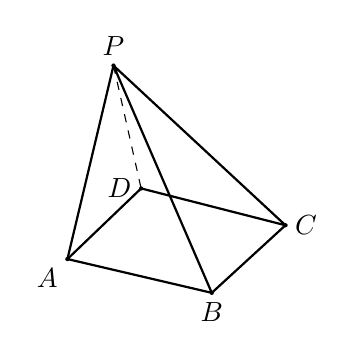
\begin{tikzpicture}[>=stealth,scale=0.78]
  \coordinate (A) at (0,0); \coordinate (B) at (2.35,-0.55);
  \coordinate (C) at (3.55,0.55); \coordinate (D) at (1.2,1.15);
  \coordinate (P) at (0.75,3.15);
  \draw[thick] (A)--(B)--(C)--(D)--cycle;
  \draw[thick] (P)--(A) (P)--(B) (P)--(C);
  \draw[dashed] (P)--(D);
  \fill (P) circle (1pt) node[above] {$P$};
  \fill (A) circle (1pt) node[below left] {$A$};
  \fill (B) circle (1pt) node[below] {$B$};
  \fill (C) circle (1pt) node[right] {$C$};
  \fill (D) circle (1pt) node[left] {$D$};
\end{tikzpicture}
\end{center}
\nopagebreak[4]
（1） 求点 $P$ 到平面 $ABCD$ 的距离；

（2） 求面 $APB$ 与面 $CPB$ 所成二面角的大小。

\Needspace{4\baselineskip}
\textbf{解析}

\gksubpart{(1)}

\Needspace{5\baselineskip}
建立空间直角坐标系，取

\nopagebreak[4]
\[
A=(0,0,0),\quad D=(2,0,0),\quad B=(1,\sqrt3,0),\quad C=(3,\sqrt3,0).
\]

\Needspace{5\baselineskip}
侧面 $PAD$ 为边长 2 的正三角形，且底面内的射线 $AB$ 与侧面内的射线 $AP$ 所成的截面角为 $120^\circ$，再结合 $PB\perp AD$，可取

\nopagebreak[4]
\[
P=\left(1,-\frac{\sqrt3}{2},\frac32\right).
\]

因此点 $P$ 到底面 $z=0$ 的距离为 $3/2$。

\gksubpart{(2)}

\Needspace{5\baselineskip}
对公共棱 $PB$，取两平面的法向量

\nopagebreak[4]
\[
\boldsymbol n_1=\overrightarrow{AB}\times\overrightarrow{AP}
=\left(\frac{3\sqrt3}{2},-\frac32,-\frac{3\sqrt3}{2}\right),
\]

\nopagebreak[4]
\[
\boldsymbol n_2=\overrightarrow{BC}\times\overrightarrow{BP}
=(0,-3,-3\sqrt3).
\]

\Needspace{5\baselineskip}
则

\nopagebreak[4]
\[
\frac{|\boldsymbol n_1\cdot\boldsymbol n_2|}
{|\boldsymbol n_1||\boldsymbol n_2|}
=\frac{18}{(3\sqrt7/2)\cdot6}
=\frac{2\sqrt7}{7}.
\]

所以两平面的锐角夹角为 $\arccos(2\sqrt7/7)$；若取棱锥内部二面角，则取其补角。

\gkanswer{答案（1）：点 $P$ 到平面 $ABCD$ 的距离为 $\dfrac32$}

\gkanswer{答案（2）：两平面的锐角夹角 $\theta$ 满足 $\cos\theta=\dfrac{2\sqrt7}{7}$，即 $\theta=\arccos\dfrac{2\sqrt7}{7}$；若取棱锥内部二面角，则为 $\pi-\theta$}

\end{answer}
\begin{answer}
\gksolhead{22}{}

\textbf{题目}：

已知双曲线 $C:\dfrac{x^2}{a^2}-y^2=1$（$a>0$）与直线 $l:x+y=1$ 相交于两个不同的点 $A\text{、}B$。

（1） 求双曲线 $C$ 的离心率 $e$ 的取值范围；

（2） 设直线 $l$ 与 $y$ 轴的交点为 $P$，且 $\overrightarrow{PA}=\dfrac5{12}\overrightarrow{PB}$。求 $a$ 的值。

\Needspace{4\baselineskip}
\textbf{解析}

\gksubpart{(1)}

\Needspace{5\baselineskip}
把 $y=1-x$ 代入双曲线，得

\nopagebreak[4]
\[
\left(\frac1{a^2}-1\right)x^2+2x-2=0.
\]

\Needspace{5\baselineskip}
要有两个不同交点，需 $a\ne1$ 且

\nopagebreak[4]
\[
\Delta=4+8\left(\frac1{a^2}-1\right)
=4\left(\frac2{a^2}-1\right)>0.
\]

\Needspace{5\baselineskip}
因此 $0<a<\sqrt2$ 且 $a\ne1$。双曲线的离心率为

\nopagebreak[4]
\[
e=\frac{\sqrt{a^2+1}}a.
\]

\Needspace{5\baselineskip}
它随 $a$ 增大而减小，故

\nopagebreak[4]
\[
e>\frac{\sqrt6}{2},\qquad e\ne\sqrt2.
\]

\gksubpart{(2)}

令直线上的点用横坐标参数表示，$P=(0,1)$，则点 $(x,1-x)$ 对应向量 $\overrightarrow{P(x,1-x)}=x(1,-1)$。设 $A\text{、}B$ 的横坐标为 $r\text{、}s$，由题设 $r=\dfrac5{12}s$。

\Needspace{5\baselineskip}
二次方程的根满足根和等于根积，故

\nopagebreak[4]
\[
r+s=rs,\qquad r=\frac5{12}s.
\]

\Needspace{5\baselineskip}
解得

\nopagebreak[4]
\[
r=\frac{17}{12},\qquad s=\frac{17}{5},
\]

\Needspace{5\baselineskip}
于是 $r+s=rs=289/60$。另一方面

\nopagebreak[4]
\[
r+s=-\frac{2a^2}{1-a^2},
\]

\Needspace{5\baselineskip}
所以

\nopagebreak[4]
\[
-\frac{2a^2}{1-a^2}=\frac{289}{60}
\Longrightarrow a^2=\frac{289}{169}.
\]

因 $a>0$，故 $a=17/13$。

\gkanswer{答案（1）：$e\in\left(\dfrac{\sqrt6}{2},+\infty\right)\setminus\{\sqrt2\}$}

\gkanswer{答案（2）：$a=\dfrac{17}{13}$}

\end{answer}